\documentclass[10pt]{article}
\usepackage{geometry}
\usepackage{latexsym}
\usepackage{amsmath}
\usepackage{multirow}
\usepackage{url}
\usepackage[numbers]{natbib}
\usepackage{graphicx}
\usepackage{subcaption}
\newgeometry{margin=3.40cm}

\graphicspath{{../figures/}}

\title{{\large CS224W Project Milestone} \\
  What is karma? Quantifying online influence and credibility
}
\author{Thomas Dimson \\ {\tt tdimson@cs.stanford.edu}
  \and
  Milind Ganjoo \\ {\tt mganjoo@cs.stanford.edu}
}
\date{}

\begin{document}
\maketitle

%% TODO: Write and include abstract.
%% TODO: This is the expected format:
% We expect that you have completed 60% of the project
% Provide a complete picture of your project even if certain key parts have not yet been implemented/solved.
% Include the parts of your project which have been completed so far, such as:
% * Thorough introduction of your problem
% * Review of the relevant prior work
% * Description of the data collection process
% * Description of any initial findings or summary statistics from your dataset
% * Description of any mathematical background necessary for your problem
% * Formal description of any important algorithms used
% * Description of general difficulties with your problem which bear elaboration
% Make sure to at least outline the parts which have not yet been completed so that it is clear specifically what you plan to do for the final version.
% Recommended length 3-5 pages

\section{Introduction}
Many online communities explicitly publicize the concept of \textit{karma} or
\textit{reputation} for users, computed as a sum of positive votes by other members of
the community. These explicit measures are often seen as proxies for more
intangible notions such as \textit{influence} (the ability of a member to
persuade others) and \textit{credibility} (the trustworthiness of the user as an
member of the community). In this paper, we describe the range of network
characteristics, interactions, and temporal factors that affect the accumulation
of karma points. Using this, we build a model that predicts karma values.

Our topic is motivated by the class content discussing how users evaluate
each other in social graphs. We wish to determine whether network properties of the 
\textit{interaction graph} can explain karma metrics. Our subsequent model for 
could inform a general framework for quantifying influence and credibility
on other graphs (including those without \textit{users} as nodes).

\section{Prior Work}
Most prior literature focuses on the abstract quality of \textit{influence}.
Both \citet{bakshy2011everyone} and \citet{cha2010measuring} define
influence as the ability to generate cascades on the Twitter graph. The authors
use local feature of users (e.g. number of followers, number of tweets,
retweets, mentions) in order to predict the ability for users to generate
cascades. 

\citet{cha2010measuring} emphasizes the topic-specificity of influence -- they challenge
the notion that there is a common set of ``influentials'' who have
broad-reaching impact on online communities. Instead, they demonstrate that for
many topics, such as political events, there are special interest groups like
bloggers and politicians that see higher retweet and mention scores than the
generally popular Twitter users.

In a very recent paper, \citet{movshovitzanalysis} consider the reputation
scheme on StackOverflow (based on upvotes and accepted answers). They 
attempt to identify expert users based on their contribution
patterns and use high reputation users for validation. The authors tried many 
techniques to improve their classifier performance including PageRank and
an SVD decomposition of their interaction graphs. Notably, they find
that PageRank does not contribute significantly to their performance
and use user features such as number of answers, questions and question-answer 
rations in their final random forest model. They are
able to achieve an Area under the Curve of 81\% when classifying users
with reputations of more than 2400.


\section{Data Collection}
For our report, we will be focusing on two communities: \textbf{Hacker News}
and the \textbf{StackExchange} family of websites. On Hacker News, users submit
technology-related stories as \textit{submissions} which other users
use as an anchor to threaded discussions. A user's \textit{karma} is computed
as a sum of up-votes to their stories and comments. The StackExchange family of 
websites are question-and-answer sites where a user will post a question and
solicit answers from the community. A user's \textit{reputation} is a weighted
sum based on the number of their questions and answers that are accepted, and
whether their comments and posts are voted as helpful by the community.

Gathering data for Hacker News came with many challenges: there is no published
dump of hacker news data, and no official API to help fetch. Fortunately, the creator
of ThriftDB has created HNSearch (\url{https://www.hnsearch.com/}) as a technology
demo for his database. In addition to a public website, there is an unofficial API
to support mechanical search queries. Although the API is limited to collecting 
only 100 recent items, we were able to circumvent this by constructing queries with limited
date ranges. Over the course of a week, we extracted JSON files for every comment,
submission and user on Hacker News by repeatedly querying the API. To our knowledge,
ours is the only complete dump of this data available on the internet.

%Milind can you talk about using SuperUser as a starting point, as well as discussing how
% you collected data. I think it is fine for this to be smaller than HN the dump is published

After collecting the raw data for both datasets, we created an SQLite database
with normalized columns for all the fields. We also created an interaction graph
by collecting $(\text{replier}, \text{parent poster})$ edges and then caching the graphs
on disk as a NetworkX structure. A summary of our datasets is available in 
Table~\ref{tab:graphstats}.

As a final step, we divided each dataset into train, validation and test sets at
a 70\%/15\%/15\% split. Our milestone results are reported on our validation
set.

\section{Initial Findings}

\begin{figure}[h]
\centering
\begin{subfigure}{0.49\textwidth}
\centering
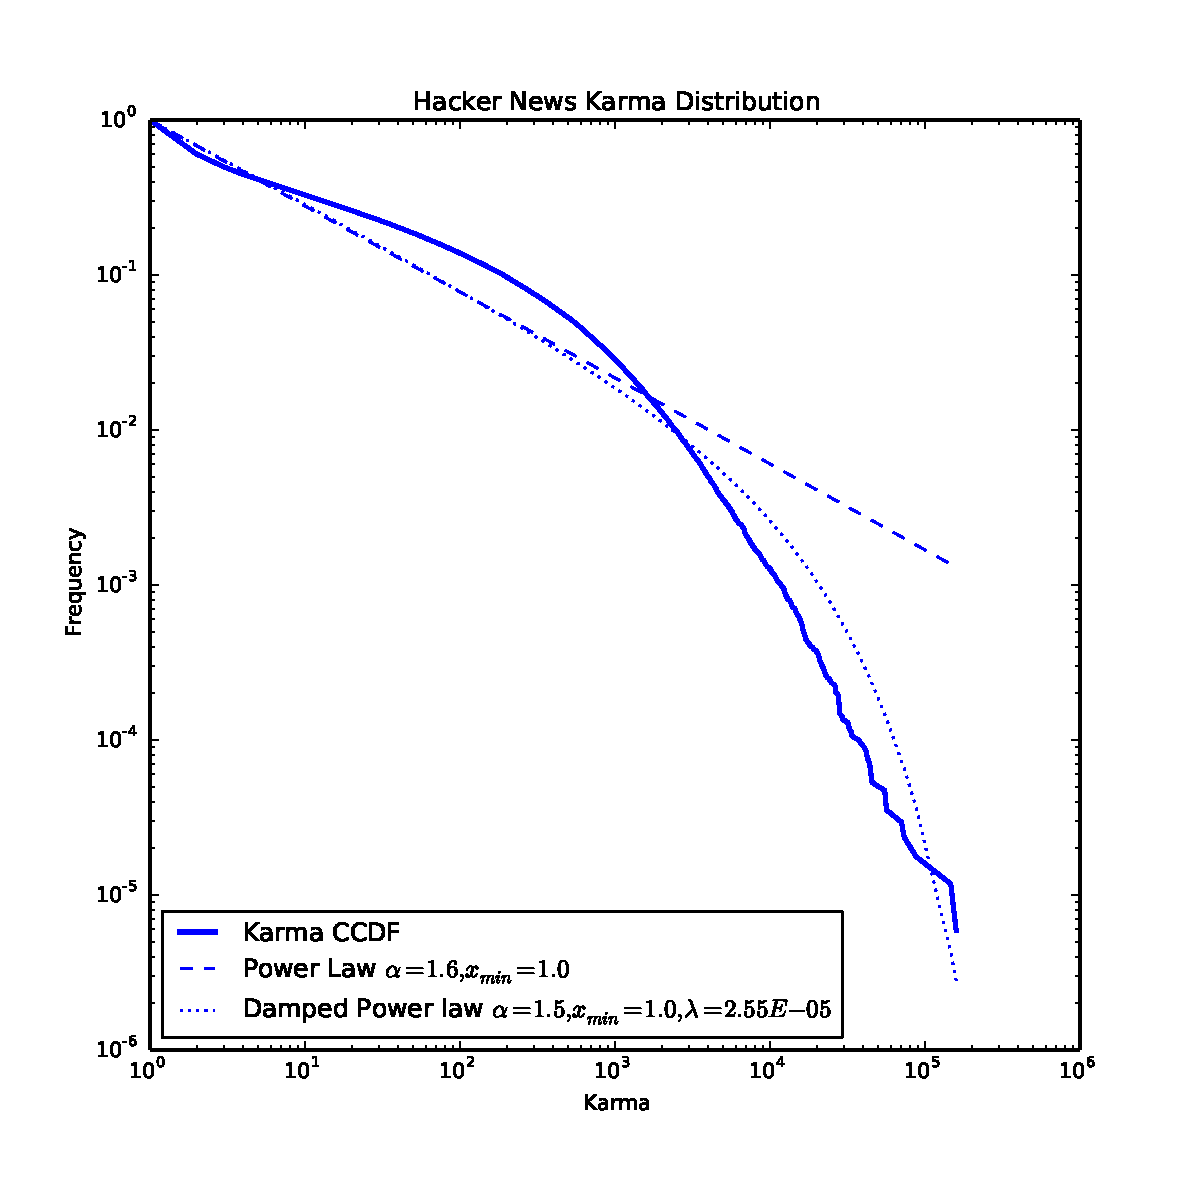
\includegraphics[width=\linewidth]{hn_karma_distribution}
\caption{Hacker News}
\label{fig:hnkarma}
\end{subfigure}%
\begin{subfigure}{0.49\textwidth}
\centering
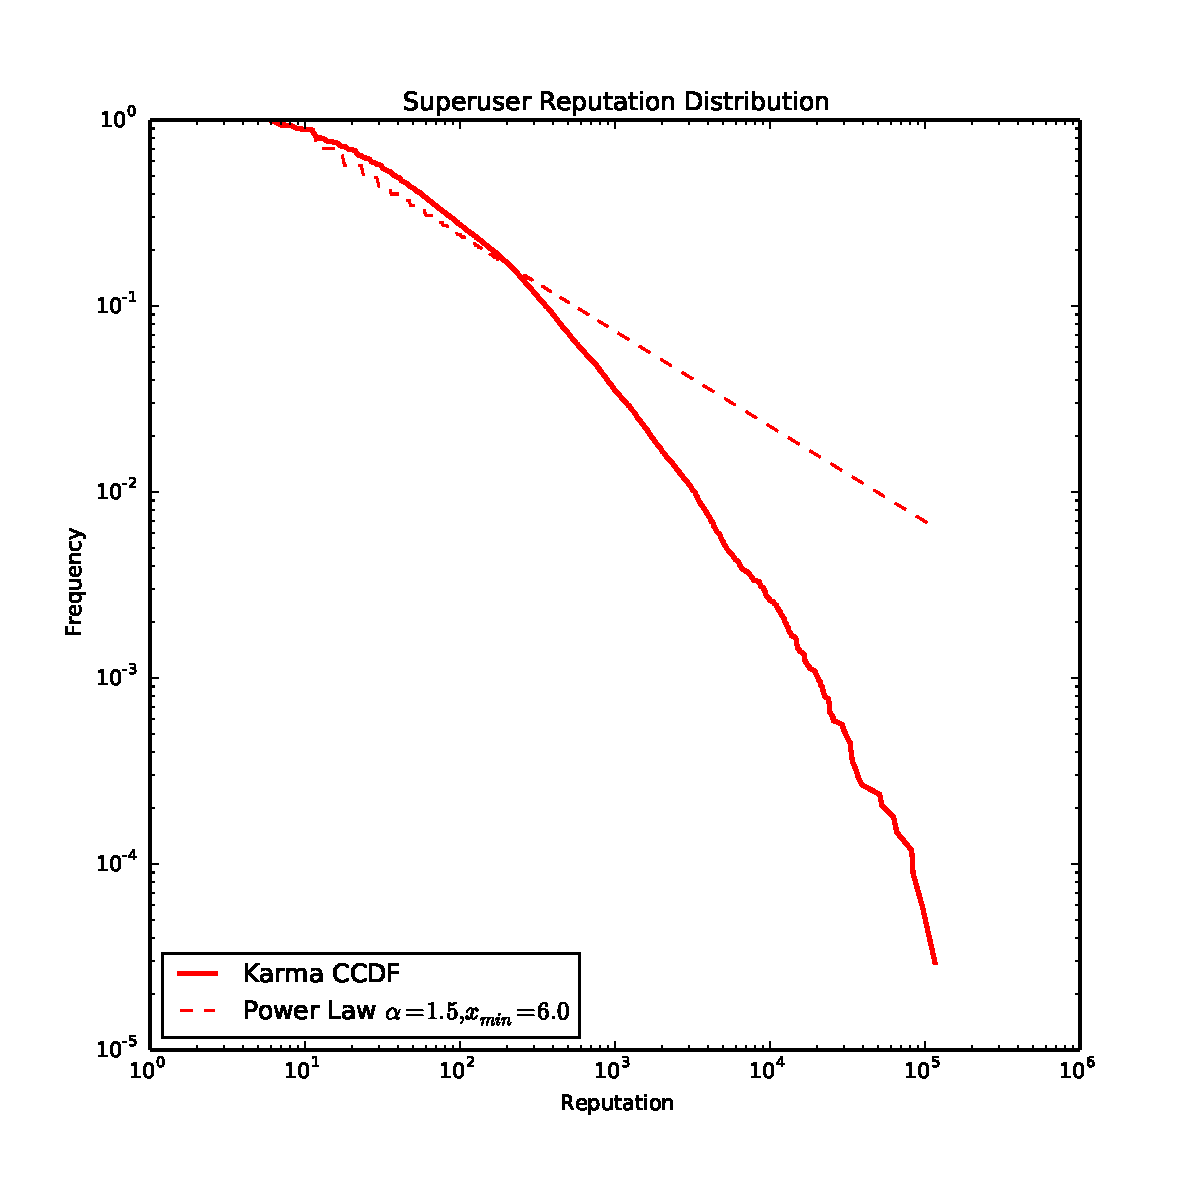
\includegraphics[width=\linewidth]{su_karma_distribution}
\caption{Super User}
\label{fig:sukarma}
\end{subfigure}
\caption{Karma distributions in our datasets with fitted power law distributions}
\label{fig:karma}
\end{figure}

We begin our data analysis with a plot of the complementary cumulative
distributinos of karma and reputations 
over users as shown in Figure~\ref{fig:karma}. As expected, both Hacker News
and Super User distributions are well-modelled power-law variants. Using 
Python's Powerlaw package~\cite{alstott_powerlaw:_2013} we also show fitted
models. Both models have an $\alpha$ coefficient near 1.5 and begin near
the origin. Notably, a damped power law is a better fit than
a power law on our Hacker News distribution and the reverse is true for
our Super User reputation distribution. Our acting hypothesis is that
Hacker News is an older community (circa 2007) with a few early adopters with incredibly
high karma while Super User is relatively new (circa 2011) that split off
of the existing StackOverflow community. 

Aligning with our karma distributions, Table~\ref{tab:graphstats} shows
interaction graph statistics for both communities. Although they are roughly
commensurate in users, Hacker News has an order of magnitude more edges in the
graph due to the threaded nature of discussions. The disparity between the
communities increases when we begin to look at strongly connected components
(SCCs): over 40\% of Hacker News members are part of their largest SCC while only
3.8\% of Super User members are part of their largest SCC. This reflects the
fact that the Q\&A site has fewer ``spanning'' conversations and a much looser
graph structure. 

In general, we are seeing that the notation of \textit{reputation} on
Super User and \textit{karma} on Hacker News are more disparate than we first
thought.

\begin{table}[h]
\begin{center}
\begin{tabular}{| r | l l |}
\hline
& \textbf{Hacker News} & \textbf{Super User} \\
\hline
Users (Nodes) & 175091 & 190781 \\
Replies (Edges) & 2747966 & 266673 \\
Average Karma / Reputation & 131.8 & 83.1 \\
Largest SCC Fraction & 43\% & 3.8\% \\
Largest WCC Fraction & 63\% & 46\% \\
\hline
\end{tabular}
\end{center}
\caption{Graph statistics for our implied interaction graphs}
\label{tab:graphstats}
\end{table}


\section{Baseline Predictor}
\label{sec:baseline}

\begin{table}[h]
\begin{center}
\begin{tabular}{| r | l l l l |}
\hline
&  \multicolumn{2}{l}{\textbf{Hacker News}} & \multicolumn{2}{l |}{\textbf{Super
User}} \\
Model & RMSE & $R^2$ & RMSE & $R^2$ \\
\hline
Baseline & 545.85 & 0.55 & 212.72 & 0.93 \\
Baseline+PageRank & 475.59 & 0.66 & 210.02 & 0.93 \\
Baseline+Weighted PageRank & \textbf{407.19} & \textbf{0.75} & \textbf{209.32} & \textbf{0.93} \\
\hline
\end{tabular}
\end{center}
\caption{Regression performance for our baseline and improved baseline models.}
\label{tab:regression}
\end{table}
% Milind, if you take a pass I'll take a pass

\subsection{Weighted PageRank}
As discussed in Section~\ref{sec:baseline}, we noticed a substantial improvement
when switching from vanilla PageRank to a weighted variant. Here, we modify
our random walk so that instead of following outbound edges uniformly at random
we sample from a weighted distribution:
\begin{align}
P(i\rightarrow j)  &= \frac{\text{Num Replies}\ i \rightarrow j}{\sum_k \text{Num
replies}\ i \rightarrow k}
\end{align}
This captures the intuition that ``deeper'', multi-commented discussions
between two users are more important than one-off replies.

\section{Next steps}
% Milind zone - cite LDA?
Latent Dirichlet Allocation (LDA) \citep{blei2003latent}. 

Going deeper, we could combine our
LDA-topic analysis with PageRank by performing Topic-Sensitive PageRank
\citep{haveliwala2002topic} on our nodes and seeing if graph authority is more
predictive of karma within certain topics. This hypothesis was validated in
predicting following relationships on the Twitter graph in
\citet{weng2010twitterrank}

\section{Conclusion}
% Milind zone

\bibliographystyle{abbrvnat}
\bibliography{milestone}

\end{document}
